% !TEX root = ../master-thesis.tex




% \beg\textbf{in{figure}
%     \centering
%     \addletter{85}{a} \phantom{4}
%     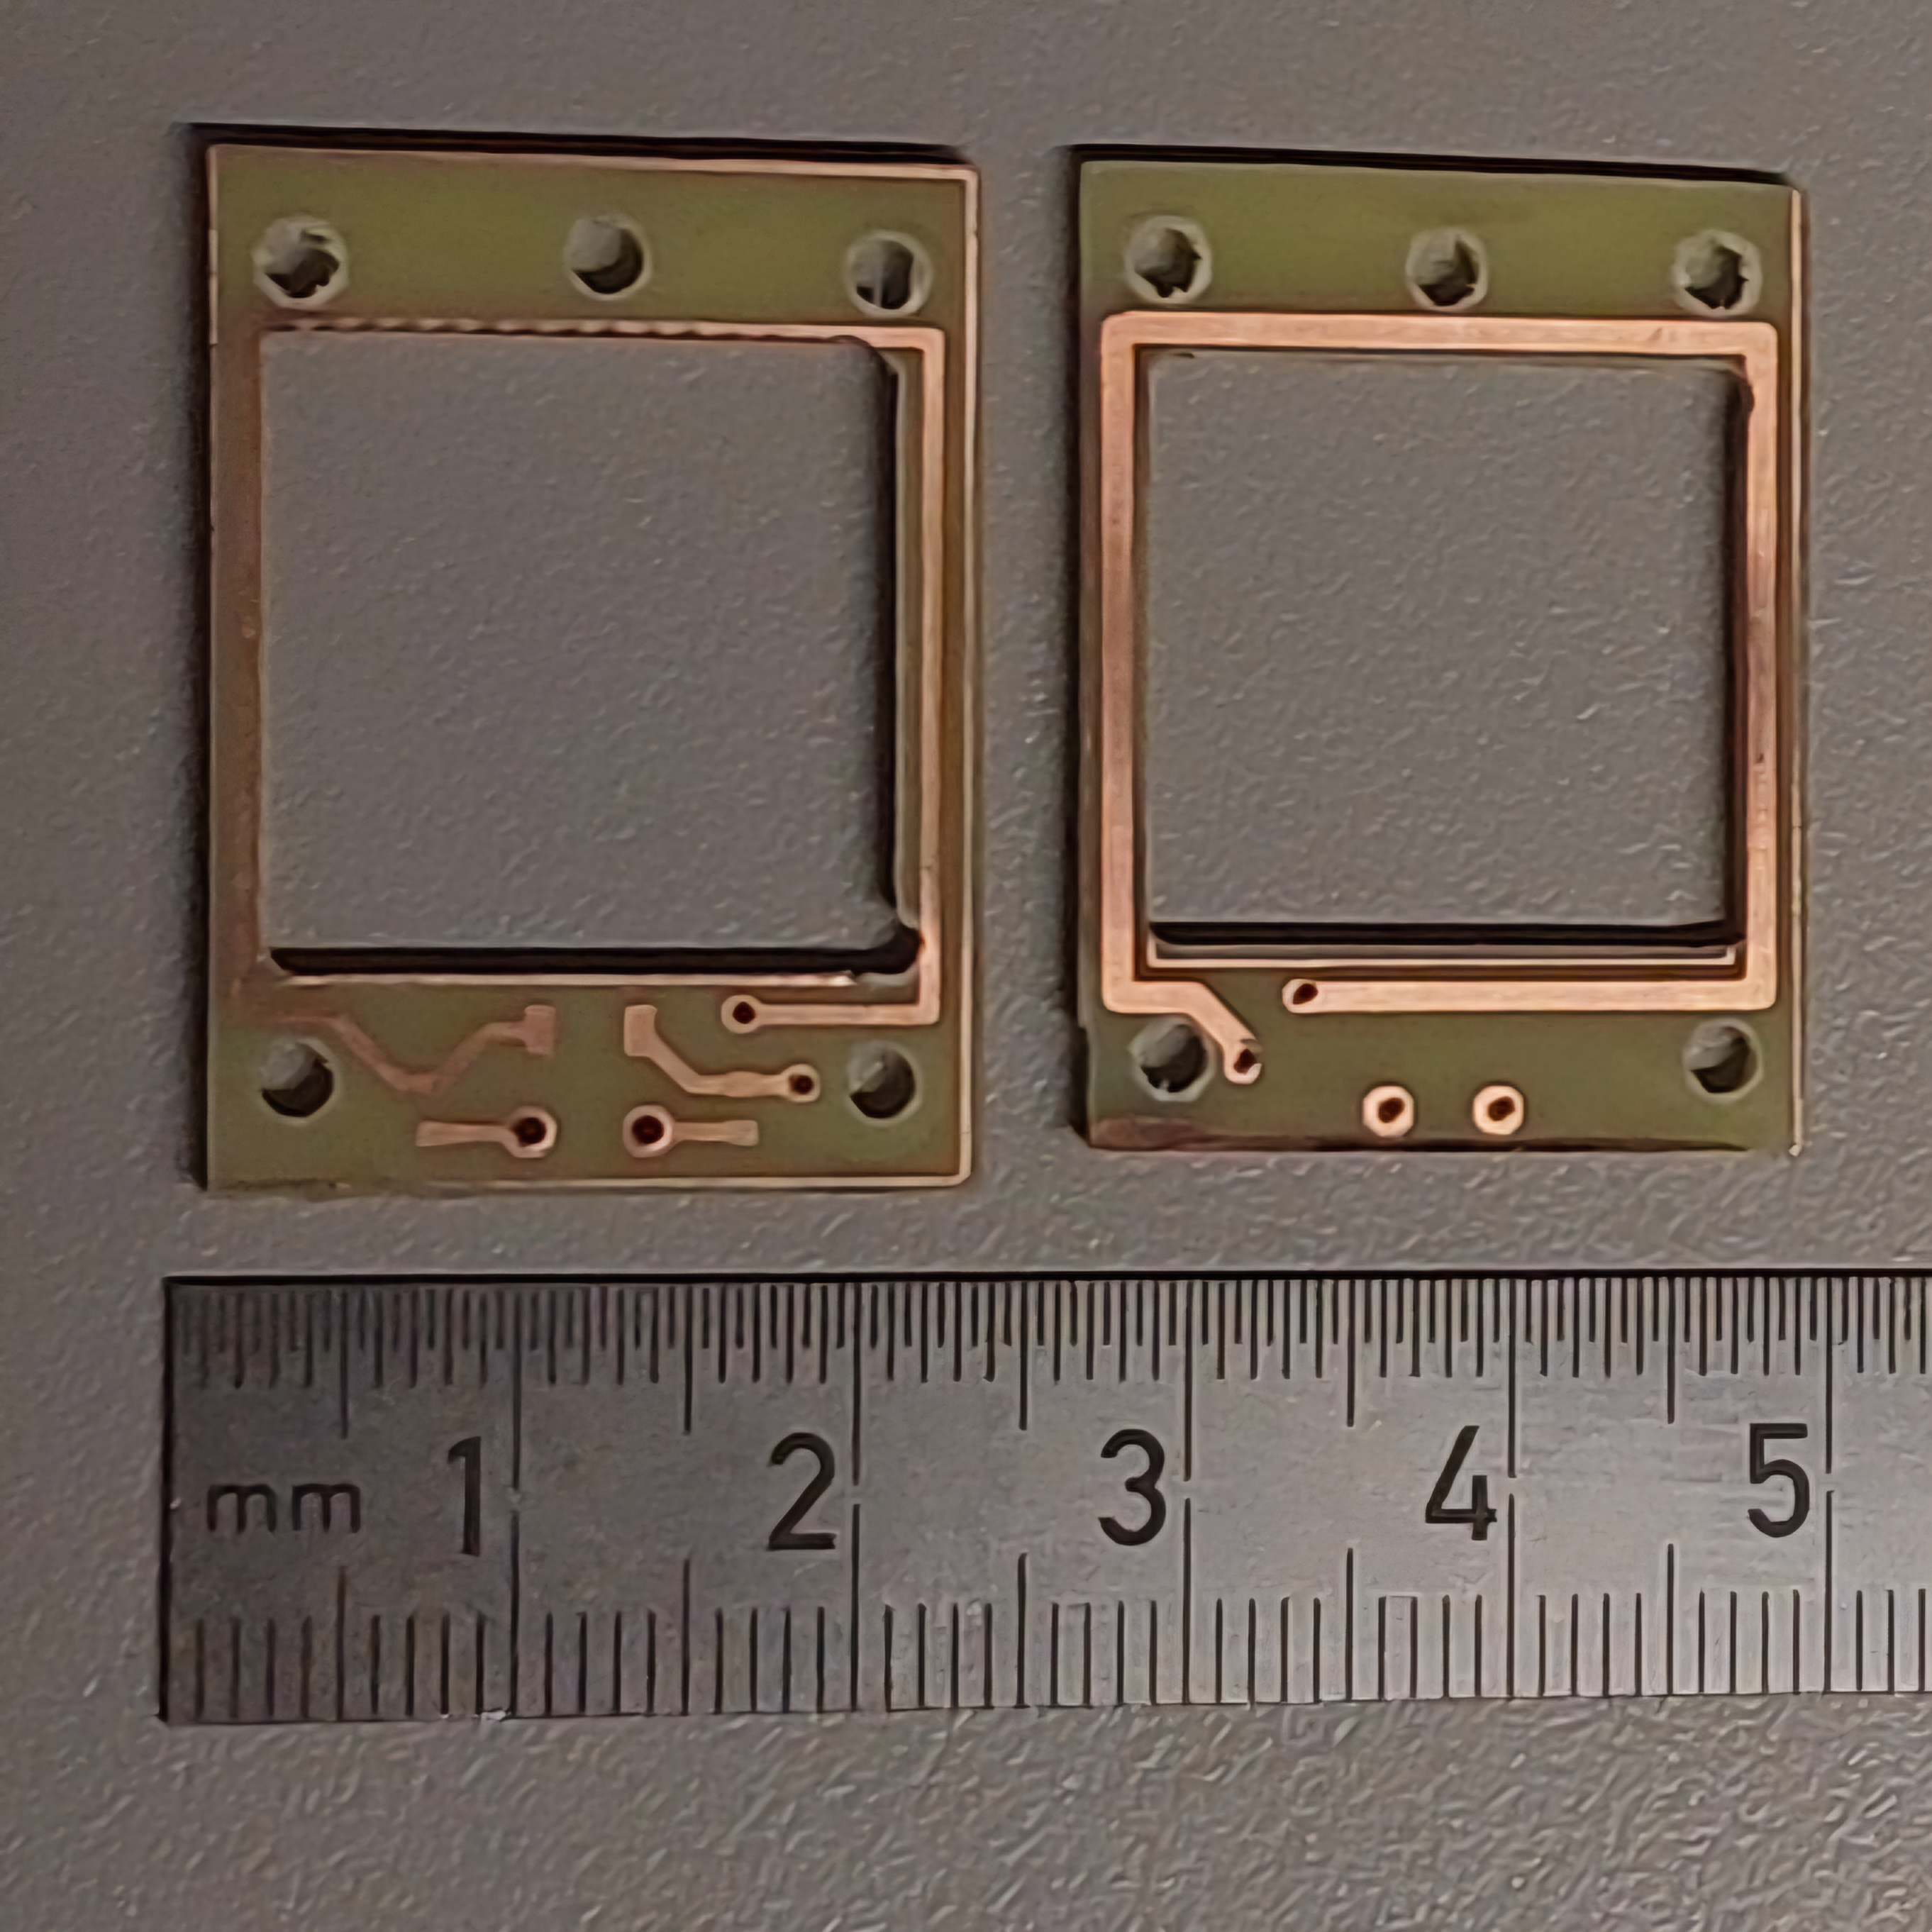
\includegraphics[width=1.25in]{imgs/RF.jpg}
%     \hspace{1cm}
%     \addletter{85}{b} \phantom{4}
%     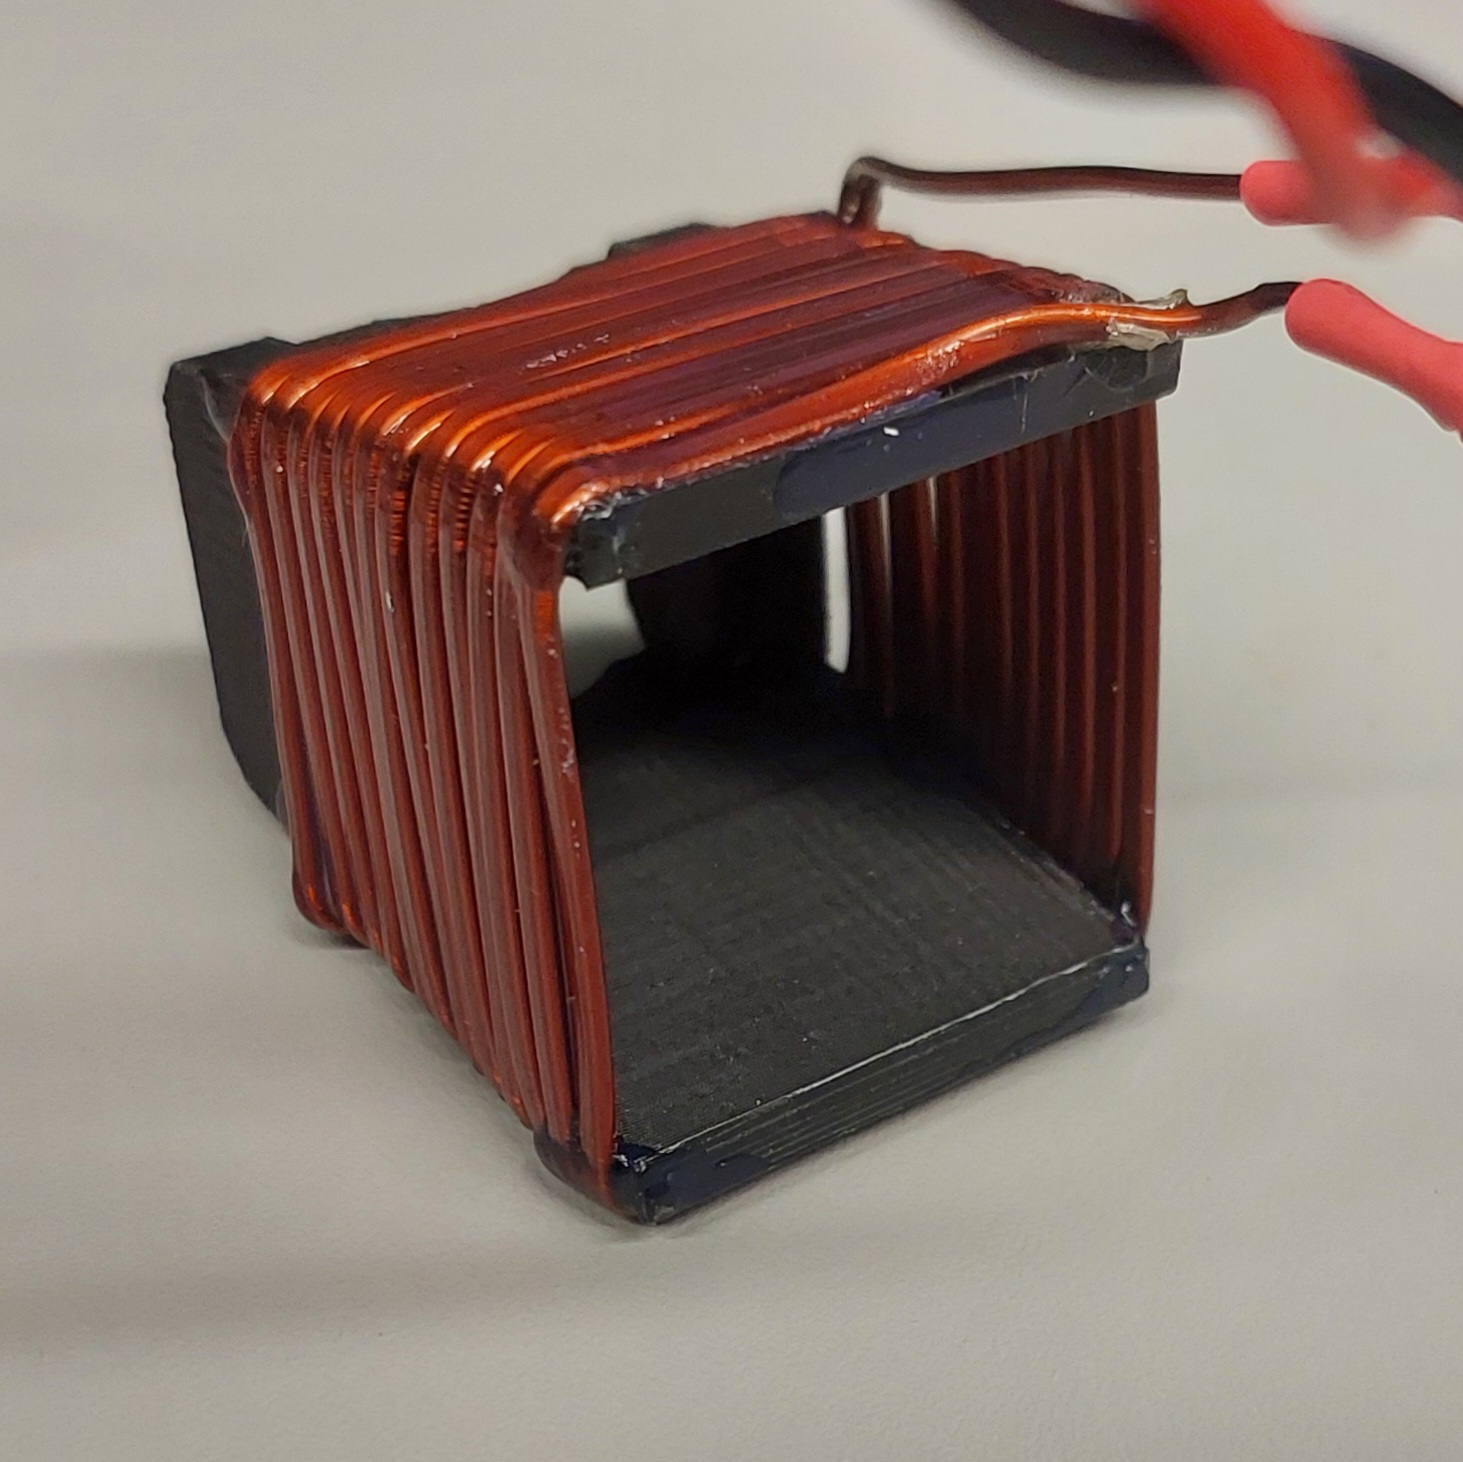
\includegraphics[width=1.25in]{imgs/MW.jpg}
%     \caption{
%         \textbf{RF and MW antennas used for spin control.}
%         (a) PCB-based radiofrequency (RF) antenna used for driving spin transitions at MHz frequencies. 
%         (b) Microwave (MW) loop antenna, designed to efficiently couple to hyperfine transitions in $^6$Li. 
%         These antennas are used for coherent spin manipulation. 
%         % performance characterization via spin-flip fidelity is discussed in the following figures.
%     }
%     \label{fig:rfmw}
% \end{figure}}


